%%%%%%%%%%%%%%%%%%%%%%%%%%%%%%%%%%%%%%%%%%%%%%%%%%%%%%%%%%%%%%%%%%%%%%%%%%%%%%%%
\section{Experiments}\label{sec:imag_coll_experiments}
%%%%%%%%%%%%%%%%%%%%%%%%%%%%%%%%%%%%%%%%%%%%%%%%%%%%%%%%%%%%%%%%%%%%%%%%%%%%%%%%
In this section we provide a number of experiments that demonstrate the
advantage of our coarse alignment and the single template recovered by our
coarse alignment scheme. We also provide experiments that emphasise the increased
robustness of our reconstructions over the least-squares solution of
\citet{KemelmacherShlizerman:2013iv}. We show a new application to this type
of model that involves improving the fitting results of an 
AAM~\cite{cootes2001active} using our
constructed SH basis. 

Choosing the number of components, $k$, to recover is an
important problem that was not properly addressed by \citet{KemelmacherShlizerman:2013iv}. 
In these experiments we attempt to recover as many
components as possible in order to strike a balance between cleanly
reconstructed normals and deformations. However, there is a trade-off when choosing
the value of $k$. In particular, if the value of $k$ is too large, then the
decomposition is unable to separate the deformation and illumination and the subspace of
illumination no longer represents valid normals. This is one of the primary advantages
of our robust decomposition, as it allows the value of $k$ to be larger given
the reduced rank of the images. However, a potential disadvantage of our
proposed method is the sensitivity of the algorithm to the parameter $\lambda$,
which must be tuned for every dataset. It is also important to stress that our
main goal is to recover the low frequency shape information to provide plausible
3D facial surfaces under challenging conditions. However, in
\cref{subsec:experiments_smith}, we show that our recovered subspace can
be used in existing high frequency recovery algorithms such as SFS.\@

The area of 3D facial surface recovery is lacking any form of formal
quantitative benchmark. The quantitative benchmark presented in
\cite{KemelmacherShlizerman:2013iv} is performed on depth data recovered from PS.\@
This is not ground truth depth data, as error is introduced during
integration, and a more accurate evaluation would be the angular error of the
recovered normals. However, in the presence of cast shadows, even the normals of
PS are biased. For this reason, the lack of a standard and fair
quantitative evaluation, we focus on qualitative results in this chapter.

Specifically we performed the following experiments:
%%%%%%%%%%%%%%%%%%%%%%%%%%%%%%%%%%%%%%%
\begin{itemize}
    \item We built our subspace using the HELEN~\cite{le2012interactive} 
          dataset. We directly compare against the least-squares decomposition
          proposed in~\cite{KemelmacherShlizerman:2013iv} and show particularly
          challenging images from the dataset. This experiment highlights the
          difficulty in constructing subspaces from large a set of
          ``in-the-wild'' images.
    \item Similar to \citet{KemelmacherShlizerman:2013iv}, we provide
          qualitative examples on shape recovery of the Yale B dataset.
    \item We show that the robust subspace learnt in (1) can be used within the
          SFS framework of \cref{sec:singl_img_gsfs}. By recovering the normals
          from every image of HELEN~\cite{le2012interactive}, we can perform a
          secondary PCA on the normals in order to directly embed them within
          the GSFS algorithm. In this experiment, we compare against a clean
          dataset of normals acquired from the 
          ICT-3DRFE~\cite{stratou2012exploring} database.
    \item We show how our subspace can be combined with an existing facial
    alignment algorithm, namely project-out AAMs~\cite{matthews2004active}. Our
    subspace can be used both as the appearance basis for the AAM and also as a
    methodology of recovering dense 3D shape.
\end{itemize}

In the following section we describe the construction of the bases and explain
what pre-processing was performed on each dataset.
%%%%%%%%%%%%%%%%%%%%%%%%%%%%%%%%%%%%%%%
\begin{table}
    \centering
    \begin{tabular}{lccccc}
        \toprule
        \textbf{Data}          & \textbf{Warp (s)} & \textbf{Decomposition (s)} & \textbf{Inverse Warp (s)} & \textbf{Total (s)} \\ \midrule
        HELEN (2330 images)    & 8                 & 730                        & 25                        & 763                \\
        Tom Hanks (274 images) & 1                 & 21                         & 4                         & 26                 \\  \bottomrule
    \end{tabular}
    \caption{\textbf{Training Times.} Mean training times in seconds over 10
             runs rounded to the nearest second. ``Warp'' denotes warping to the
             LFPW reference frame of $(150 \times 150)$ pixels, ``Inverse Warp''
             denotes warping back to the original images and ``Decomposition''
             denotes the total training time of our method described in
             \cref{subsec:imag_coll_robust_sh_basis}. Original images were larger than 
             the reference, hence the increase from ``Warp'' to ``Inverse Warp''.
             Timings were recorded on an Intel Xeon E5--1650 3.20GHz with
             32GB of RAM.}
\label{tbl:imag_coll_timings}
\end{table}
%%%%%%%%%%%%%%%%%%%%%%%%%%%%%%%%%%%%%%%
%%%%%%%%%%%%%%%%%%%%%%%%%%%%%%%%%%%%%%%%%%%%%%%%%%%%%%%%%%%%%%%%%%%%%%%%%%%%%%%%
\subsection{Constructing The Robust Bases}\label{subsec:imag_coll_construction}
%%%%%%%%%%%%%%%%%%%%%%%%%%%%%%%%%%%%%%%%%%%%%%%%%%%%%%%%%%%%%%%%%%%%%%%%%%%%%%%%
The process of building the robust SH basis was the same for all datasets
involved. Facial annotations consisting of 68 points were recovered through
various methods for each dataset. In the case of the 
HELEN~\cite{le2012interactive} database, the manual
annotations provided by the IBUG group were used~\cite{sagonas2013300,sagonas2013semi},
in the case of the Yale B, Photoface and ICT-3DRFE databases, manual annotations
were used and the ``in-the-wild'' images and video of Tom Hanks were automatically
annotated by the one millisecond facial alignment method of~\cite{kazemi2014one}
provided by the Dlib project~\cite{king2009dlib}.

These annotations were then warped via a Piecewise Affine transformation to a
mean reference shape that was built from all the faces, training and testing, of
the LFPW~\cite{belhumeur2013localizing} facial annotations provided by 
IBUG~\cite{sagonas2013300,sagonas2013semi}.
This provided the dense
correspondence required for performing matrix decompositions. To construct our
SH bases, we performed the algorithm as described in
\cref{subsec:imag_coll_robust_sh_basis} on the warped images. In order to provide
the example reconstructions, the reconstructed images were warped back into
their original shapes and then integrated using the method of 
\citet{frankot1988method}.

\cref{tbl:imag_coll_timings} gives examples of the training time taken for the 
``in-the-wild'' Tom Hanks images and the HELEN dataset. It is important to note that
part of the reason the training time is much lower for the Tom Hanks images is
that they have an inherently lower rank than the HELEN images as they are all of
the same individual. This greatly affects the convergence time and thus the
timings do not scale linearly.
%%%%%%%%%%%%%%%%%%%%%%%%%%%%%%%%%%%%%%%%
\newcommand{\yaleb}[1]
{
\includegraphics[width=3.5cm,height=4cm]{collection_ps/images/yaleb_results/yale_b_#1}                      & \hspace{1.5cm} 
\includegraphics[width=3.5cm,height=4cm]{collection_ps/images/yaleb_results/yale_b_#1_photometric}          & \hspace{1.5cm}
\includegraphics[width=3.5cm,height=4cm]{collection_ps/images/yaleb_results/yale_b_#1_photometric_low_rank}
}
\setlength{\tabcolsep}{1pt}
\begin{figure}
    \centering
    \begin{tabular}{ccc}
        Input & \hspace{1.5cm} Photometric Stereo & \hspace{1.5cm} Proposed  \vspace*{0.2cm} \\ 
        \yaleb{B01}                            \\
        \yaleb{B03}                            \\
        \yaleb{B06}                                                  
    \end{tabular}
    \caption{{Examples comparing against traditional Photometric Stereo}. 
             Images from the Yale B dataset~\cite{georghiades2001fromfew}. 
             First column is the input images, second column is traditional 
             PS result and the third column is the proposed algorithm.}
\label{fig:imag_coll_yale_b}
\end{figure}
\setlength{\tabcolsep}{6pt}
%%%%%%%%%%%%%%%%%%%%%%%%%%%%%%%%%%%%%%%%
%%%%%%%%%%%%%%%%%%%%%%%%%%%%%%%%%%%%%%%%%%%%%%%%%%%%%%%%%%%%%%%%
\subsection{Comparison Using HELEN}\label{subsec:imag_coll_experiments_helen}
%%%%%%%%%%%%%%%%%%%%%%%%%%%%%%%%%%%%%%%%%%%%%%%%%%%%%%%%%%%%%%%%
In this set of experiments we wished to convey two results: (1) that we are
capable of quickly constructing our basis on a large number of in-the-wild
images, (2) that the our robust formulation of the problem gives superior
performance to the blind decomposition used by \citet{KemelmacherShlizerman:2013iv}. 
In this experiment, $k = 200$ and the total number of components was thus $4k = 800$.
\cref{fig:imag_coll_helen_compare} shows the results from this experiment. As we can
clearly see, on challenging images the least-squares decomposition is unable to
separate the appearance from the illumination and thus the recovered normals are
unable to recover accurate shape.

\cref{fig:imag_coll_helen_compare_morphable_model} provides three examples
of reconstructions by commercial 3DMM~\cite{volker1999morphable} systems on
some of the more challenging frames. Note that the underlying shape bares little
resemblance to the perceived shape of the face and that the algorithms are
particularly insensitive to the age of the subject. In contrast, class-specific
PS contains no shape prior that limits the variability of the recovered shape.
%%%%%%%%%%%%%%%%%%%%%%%%%%%%%%%%%%%%%%%%%%%%%%%%%%%%%%%%%%%%%%%%
\subsection{Comparison Using Yale B}\label{subsec:imag_coll_experiments_yaleb}
%%%%%%%%%%%%%%%%%%%%%%%%%%%%%%%%%%%%%%%%%%%%%%%%%%%%%%%%%%%%%%%%
In this experiment we compare the result of our proposed algorithm to 
that of traditional Photometric Stereo. In this scenario, the images are assumed
to be aligned and we do not perform any pre-processing of the images. Only the
inner facial region is considered for recovery in order to reduce noise present
in the background of the image. \cref{fig:imag_coll_yale_b} shows examples
of the results. Our proposed method is smoother than that of the least-squares
PS result as the low-rank constraint naturally removes sparse noise and
high-frequency details. For this experiment $k = 1$ as their is only a single
identity and expression present in the input images. Note that our method
shares similarities to that of \citet{wu2010robust} in this scenario as it
amounts to a robust U-PS algorithm. However, \citet{wu2010robust} do not consider
a spherical harmonic image formation model and so our proposed algorithm is
still novel. Finally, we do not directly compare against
\citet{KemelmacherShlizerman:2013iv} in this experiment as, assuming $k = 1$,
the factorisation performed is exactly that of U-PS~\cite{basri2007photometric}.
%%%%%%%%%%%%%%%%%%%%%%%%%%%%%%%%%%%%%%%%%%%%%%%%%%%%%%%%%%%%%%%%
\subsection{Using The Subspace In SFS}\label{subsec:imag_coll_experiments_smith}
%%%%%%%%%%%%%%%%%%%%%%%%%%%%%%%%%%%%%%%%%%%%%%%%%%%%%%%%%%%%%%%%
The SFS technique of \citet{smith2006recovering}, as described in
\cref{sec:singl_img_gsfs}, relies on a PCA basis
constructed from normals of a single class of object. It then seeks to recover
the high frequency normal information directly from the texture. In order to
create the PCA required by GSFS, we recovered spherical harmonics
for every image in the dataset using the proposed algorithm. We then computed
Kernel-PCA as described in \cref{subsubsec:singl_img_ca_kpca} on the normals
recovered from the HELEN images and supplied them to the GSGS framework.
The lighting vector is also an input to the algorithm and we estimate it by
solving a least-squares problem with the known mean normals.

In order to provide a comparison for our reconstruction, we created a clean
normal subspace using the data from the ICT-3DRFE~\cite{stratou2012exploring}
database. This database is primarily use for image relighting purposes, however,
they provide a very accurate set of normals of faces under a wide range of
expressions. The results of this experiment are shown in \cref{fig:imag_coll_smith}.
Although our subspace did not provide reconstructions that are as visually
accurate as the subspace from ICT-3DRFE, they were still able to successfully
recover a plausible representation of the high frequency shading information.
This demonstrates that our recovered SH subspace is yielding plausible surface
normals that are capable of constraining SFS within the space of human faces.
%%%%%%%%%%%%%%%%%%%%%%%%%%%%%%%%%%%%%%%
\begin{figure}[t]
    \centering
    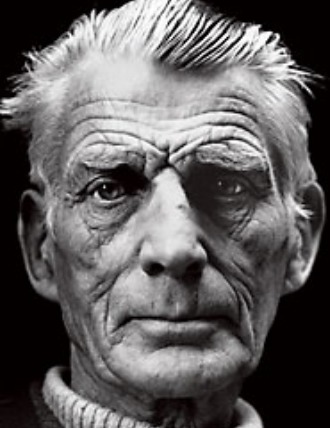
\includegraphics[width=4cm,height=4.8cm]{collection_ps/images/smith/samuel_beckett}                    \hspace{0.3cm}
    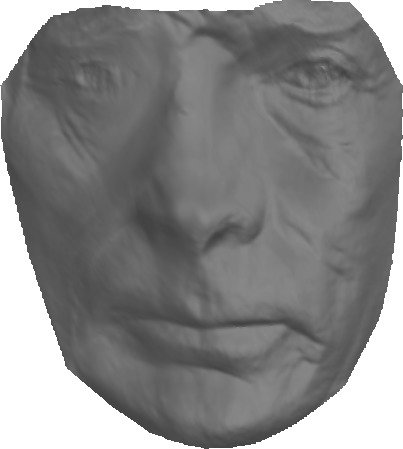
\includegraphics[width=4cm,height=4.8cm]{collection_ps/images/smith/beckett_smith_frontal_ict}         \hspace{0.3cm}
    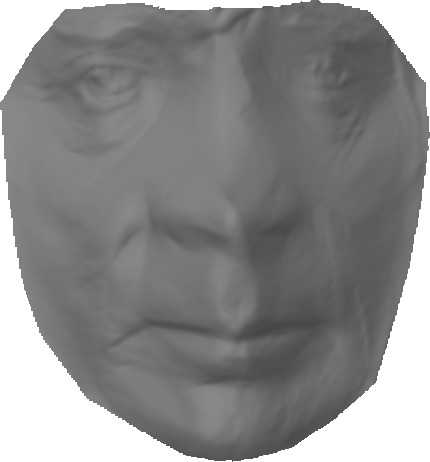
\includegraphics[width=4cm,height=4.8cm]{collection_ps/images/smith/beckett_smith_frontal_low_rank}    \\
    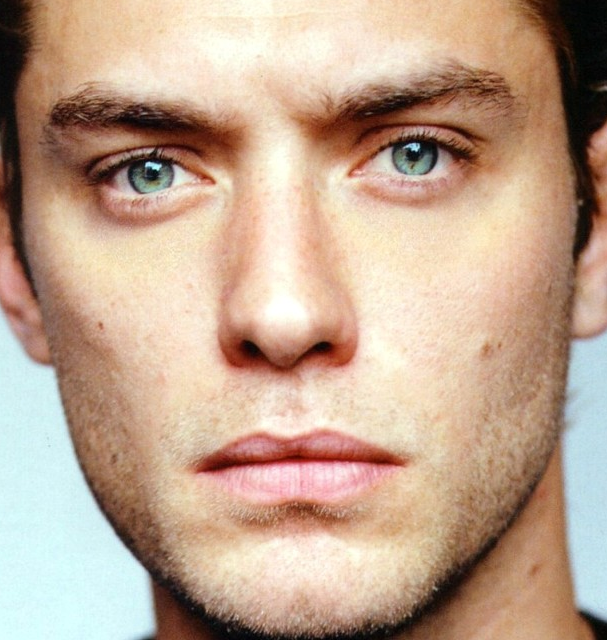
\includegraphics[width=4cm,height=4.8cm]{collection_ps/images/smith/jude_law}                          \hspace{0.3cm}
    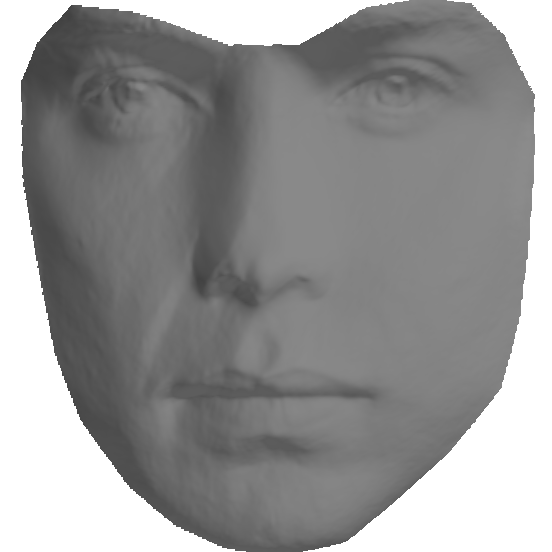
\includegraphics[width=4cm,height=4.8cm]{collection_ps/images/smith/law_smith_frontal_ict}             \hspace{0.3cm}
    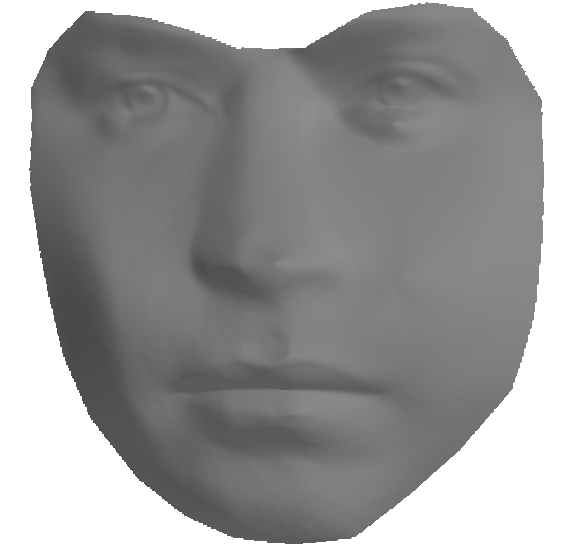
\includegraphics[width=4cm,height=4.8cm]{collection_ps/images/smith/law_smith_frontal_low_rank}
    \caption{{\bf Our subspace used for SFS}. Normals learnt automatically from 
             the Spherical Harmonic subspace of HELEN~\cite{le2012interactive} vs
             normals from the clean data of ICT-3DRFE~\cite{stratou2012exploring}.
             Middle column: the clean data. 
             Right column: proposed subspace.}
\label{fig:imag_coll_smith}
\end{figure}
%%%%%%%%%%%%%%%%%%%%%%%%%%%%%%%%%%%%%%%
%%%%%%%%%%%%%%%%%%%%%%%%%%%%%%%%%%%%%%%%%%%%%%%%%%%%%%%%%%%%%%%%
\subsection{Automatic Alignment}\label{subsec:experiments_alignment}
%%%%%%%%%%%%%%%%%%%%%%%%%%%%%%%%%%%%%%%%%%%%%%%%%%%%%%%%%%%%%%%%
%%%%%%%%%%%%%%%%%%%%%%%%%%%%%%%%%%%%%%%
\newcommand{\tomhanksalignment}[1]
{
\includegraphics[width=3.5cm]{collection_ps/images/tom_hanks/tom_hanks_improve_#1_initial} &
\includegraphics[width=3.5cm]{collection_ps/images/tom_hanks/tom_hanks_improve_#1_final}   & \hspace{0.2cm}
\includegraphics[width=3.5cm,height=3.3cm]{collection_ps/images/tom_hanks/tom_hanks_improve_#1_depth}
}
%%%%%%%%%%%%%%%%%%%%%%%%%%%%%%%%%%%%%%%
%%%%%%%%%%%%%%%%%%%%%%%%%%%%%%%%%%%%%%%
\setlength{\tabcolsep}{1pt}
\begin{figure}
    \centering
    \begin{subfigure}[b]{0.65\textwidth}
        \centering
        \begin{tabular}{ccc}
            Initial & Final & \hspace{0.2cm} Recovered Depth \\
            \tomhanksalignment{1}                            \\
            \tomhanksalignment{129}
        \end{tabular}
        \caption{}
\label{subfig:imag_coll_improve_tom_hanks_recovered}
    \end{subfigure}
    \hspace{0.1cm} \vrule \hspace{0.1cm}
    \begin{subfigure}[b]{0.25\textwidth}
        \centering
        \begin{tabular}{c}
            Improvement \\
            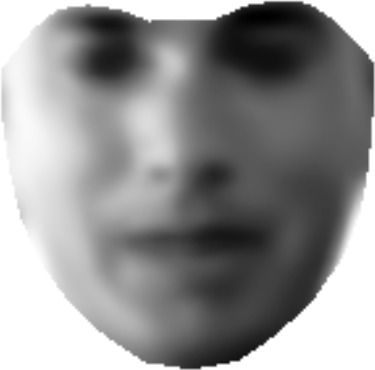
\includegraphics[width=3.5cm]{collection_ps/images/tom_hanks/tom_hanks_improve_0_initial} \\
            
\includegraphics[width=3.5cm]{collection_ps/images/tom_hanks/tom_hanks_improve_10_final}
        \end{tabular}
        \caption{}
\label{subfig:imag_coll_improve_tom_hanks_improve}
    \end{subfigure}
    \caption{{\bf Person specific model fitting for Tom Hanks.} Images of Tom 
             Hanks coarsely aligned by a facial alignment method. Our algorithm 
             improves the facial alignment and simultaneously recovers depth. 
             Images shown are from a YouTube video of Tom Hanks. 
             \cref{subfig:imag_coll_improve_tom_hanks_recovered} shows the
             recovered depth and improved landmarks from the person specific
             fitting. 
             \cref{subfig:imag_coll_improve_tom_hanks_improve} shows the
             improvement to the mean of all frames after the first iteration
             (top row) and after the final (10th) iteration (bottom row).}
\label{fig:imag_coll_improve_tom_hanks}
\end{figure}
\setlength{\tabcolsep}{6pt}
%%%%%%%%%%%%%%%%%%%%%%%%%%%%%%%%%%%%%%%
%%%%%%%%%%%%%%%%%%%%%%%%%%%%%%%%%%%%%
\newcommand{\tomhanks}[1]
{
\includegraphics[width=2.7cm,height=3.2cm]{collection_ps/images/tom_hanks/tom_hanks_#1}                   &
\includegraphics[width=2.7cm,height=3.2cm]{collection_ps/images/tom_hanks/tom_hanks_#1_low_rank}          & 
\includegraphics[width=2.7cm,height=3.2cm]{collection_ps/images/tom_hanks/tom_hanks_#1_low_rank_textured}
}
%%%%%%%%%%%%%%%%%%%%%%%%%%%%%%%%%%%%%
%%%%%%%%%%%%%%%%%%%%%%%%%%%%%%%%%%%%%
\setlength{\tabcolsep}{1pt}
\begin{figure}
    \centering
    \begin{tabular}{cccccc}
        Input & Shape & Textured & Input & Shape & Textured \vspace*{0.2cm} \\ 
        \tomhanks{14}            & \tomhanks{27}                            \\
        \tomhanks{95}            & \tomhanks{52}
    \end{tabular}
    \caption{{\bf Example reconstructions of Tom Hanks}. Images automatically 
             downloaded from Google Images. First column is the input images, 
             second column is the untextured shape from the proposed technique 
             and the third column is the textured shape.}
\label{fig:imag_coll_tom_hanks}
\end{figure}
\setlength{\tabcolsep}{6pt}
%%%%%%%%%%%%%%%%%%%%%%%%%%%%%%%%%%%%%
In this experiment we use a variation of the traditional AAM~\cite{cootes2001active}
algorithm that is equivalent to the project-out algorithm as proposed by
\citet{matthews2004active}. Practically, we
used the Active Template Model (ATM) provided by the Menpo
project~\cite{menpo14} in order to perform a project-out type algorithm to align
images of Tom Hanks. This model is similar to the Lucas-Kanade
\cite{lucas1981iterative} method but uses a point distribution model (PDM) in order to
perform non-rigid alignment between the images. In particular, the template
image is fixed during optimisation of the PDM, and we use our subspace to
provide a texture representing an approximation of the diffuse component of the
image. This is essentially identical to the procedure performed within a
project-out AAM.\@

We used a person specific SH subspace that was built on images of Tom Hanks that
were downloaded automatically from the Internet. In this case, the images were
automatically aligned using the DLib implementation of~\cite{kazemi2014one}. For
this experiment, $k = 30$ and thus the total number of components $4k = 120$.
Example reconstructions of this person specific SH basis are given in
\cref{fig:imag_coll_tom_hanks} where the output shapes bear a strong resemblance
to Tom Hanks despite the mixture of ages present in the images.

We downloaded 200 frames from a Youtube video of Tom
Hanks\footnote{\url{https://www.youtube.com/watch?v=nFvASiMTDz0} from 3:43} and
attempted to automatically align them using our subspace and the ATM.\@ The ATM
was initialised using the fitting of~\cite{kazemi2014one} and was then
iteratively improved. At each global iteration, we recovered a new set of
diffuse textures for each frame and then performed a refitting of every frame.
This caused the images to align over a sequence of iterations. We performed 10
such iterations. \cref{subfig:imag_coll_improve_tom_hanks_recovered} shows two
example frames where the alignment was improved and dense shape was also
recovered. \cref{subfig:imag_coll_improve_tom_hanks_improve} shows the
improvement in alignment over the global iterations. The final iteration is much
sharper than the initial iteration which demonstrates that the correspondence
across all frames has been visibly improved.
%%%%%%%%%%%%%%%%%%%%%%%%%%%%%%%%%%%%%%%%
\newcommand{\comparemm}[1]
{
\includegraphics[width=3cm,height=3.5cm]{collection_ps/images/helen/helen_#1}                 & \hspace{0.2cm}
\includegraphics[width=3cm,height=3.5cm]{collection_ps/images/helen/helen_#1_frontal_vizago}  & \hspace{0.2cm}
\includegraphics[width=3cm,height=3.5cm]{collection_ps/images/helen/helen_#1_side_vizago}     & \hspace{0.2cm}
\includegraphics[width=3cm,height=3.5cm]{collection_ps/images/helen/helen_#1_frontal_facegen} & \hspace{0.2cm}
\includegraphics[width=3cm,height=3.5cm]{collection_ps/images/helen/helen_#1_side_facegen}
}
\setlength{\tabcolsep}{1pt}
\begin{figure*}
    \centering
    \begin{tabular}{ccccc} \vspace*{0.2cm}
        Input & \multicolumn{2}{c}{vizago.ch} & \multicolumn{2}{c}{facegen.com}  \\
        \comparemm{6}                                                            \\
        \comparemm{680}                                                          \\
        \comparemm{821}                  
    \end{tabular}
    \caption{{\bf Examples of difficult reconstructions for existing commercial 
              Morphable Model implementations}. 
             Images from the HELEN~\cite{le2012interactive} dataset. 
             Both implementations do not provide the ability to render 
             textureless surfaces.
             Facegen.com reported invalid landmarks for the image given in the
             first row.}
\label{fig:imag_coll_helen_compare_morphable_model}
\end{figure*}
\setlength{\tabcolsep}{6pt}
%%%%%%%%%%%%%%%%%%%%%%%%%%%%%%%%%%%%%%%%
%%%%%%%%%%%%%%%%%%%%%%%%%%%%%%%%%%%%%%%%
\newcommand{\comparehelen}[2]
{
\includegraphics[width=2.5cm,height=2.5cm]{collection_ps/images/helen/helen_#1}                  & \hspace{0.5cm}
\includegraphics[width=2.3cm,height=2.5cm]{collection_ps/images/helen/helen_#1_frontal_low_rank} & \hspace{0.5cm}
\includegraphics[width=2.3cm,height=2.5cm]{collection_ps/images/helen/helen_#1_frontal_ira}      & \hspace{0.5cm}
\includegraphics[width=3cm,height=2.5cm]{collection_ps/images/helen/helen_#1_#2_low_rank}        & \hspace{0.5cm}
\includegraphics[width=3cm,height=2.5cm]{collection_ps/images/helen/helen_#1_#2_ira}
}
\begin{landscape}
\thispagestyle{footeronly}
\setlength{\tabcolsep}{1pt}
\begin{figure*}
    \centering
    \begin{tabular}{ccccc} \vspace*{0.2cm}
        Input & \hspace{0.5cm} Proposed & \hspace{0.5cm}~\cite{KemelmacherShlizerman:2013iv} & \hspace{0.5cm} Proposed & \hspace{0.5cm}~\cite{KemelmacherShlizerman:2013iv} \\
        \vspace*{-0.1cm}
        \comparehelen{1348}{side} \\ \vspace*{-0.07cm}
        \comparehelen{555}{side}  \\ \vspace*{-0.07cm}
        \comparehelen{680}{chin}  \\ \vspace*{-0.07cm}
        \comparehelen{6}{chin}    \\ \vspace*{-0.07cm}
        \comparehelen{821}{side}  \\ \vspace*{-0.07cm}
        \comparehelen{77}{side}                                      
    \end{tabular}
    \caption{{\bf Comparison with the least-squares decomposition 
             of~\cite{KemelmacherShlizerman:2013iv}}.
             Images from the HELEN~\cite{le2012interactive} dataset.}
\label{fig:imag_coll_helen_compare}
\end{figure*}
\setlength{\tabcolsep}{6pt}
\end{landscape}
%%%%%%%%%%%%%%%%%%%%%%%%%%%%%%%%%%%%%%%%
